\chapter{Completed Work}


This work was published at Physical Review E \cite{de_leeuw_diffusion_2012},
and reprinted here in \autoref{sec:papers}. In the
following sections we will provide an overview
of the main results.


%%%%%%%%%%%%%%   Overview over article should not include too much equations
%%  bottom line - take home message - the derivations should ref the article

%%  
%%  remove the techinalities - 
%%     using the procedure we have calculated for.. blah blah
%%       see figure. (leave plots only if neccessary to buttom line).
%%
%%  geometry plots - maybe try with normal scale.
%%                   if that doesn't work, leave the figure out.



%%%%%%%%%%%%%%%%%%%%%%%%%

%%%%%%%%%%%%%
%\section{Article abstract}
%\rmrk{This is the article abstract..}


We have studied random networks whose dynamics are
described by a rate equation, with transition rates $w_{nm}$
that form a symmetric matrix (\autoref{sec:matrices}),
with a diagonal conforming to \autoref{eq:zero_sum}. 
%
The long time evolution
of the system is characterized by a diffusion coefficient~$D$.
In one dimension it is well known that $D$ can display an abrupt
percolation-like transition from diffusion (${D>0}$)
to sub-diffusion (${D=0}$). 
%
A question arises whether
such a transition happens in higher dimensions.
Numerically $D$ can be evaluated using a resistor network
calculation, or optionally it can be deduced from 
the spectral properties of the system. 
%
Contrary to a recent 
expectation that is based on a renormalization-group analysis, 
we deduce that $D$ is finite,
%
suggest an ``effective-range-hopping'' procedure to evaluate $D$,
which describes the crossover between linear behavior and the \emph{VRH}
estimate.
The same approach is useful for the analysis of 
networks that are described by quasi-one-dimensional  
sparse banded matrices. 


%%%%%%%%%%%%%%%%%%%%%%%%%
\section{The effective range hopping procedure}

This is a refinement of the well established combination
of the \emph{VRH} method and a percolation threshold
 \cite{miller_impurity_1960,ambegaokar_hopping_1971,halperin_remarks_1989,pollak_percolation_1972}.


The basic idea behind \emph{ERH} (effective range hopping) is that in the linear
expression, nearby sites 
with $r\ll 1$ (and therefore $w \gg 1$ ) are over represented in
the diffusion coefficient calculation. While the transition to
these sites is indeed high, the distance covered is not enough
to form a percolating cluster. Therefore, we use a threshold based
on percolation theory and flat-down the rates higher then this threshold.
This produces a smooth crossover between the linear
estimate and the \emph{VRH} estimate.
Using the \emph{ERH} procedure we have calculated the diffusion for 
several models.


The first two models have sites randomly scattered 
in space, with average distance $r_0$, and rates $w_{nm} = w_0\eexp{-\epsilon_{nm}} \exp[-\frac{r_{nm}}{\xi}]$.


In the degenerate hopping model with $\epsilon_{nm} =0$ the \emph{ERH} result gives:

\begin{align}
D_{\tbox{ERH}} \ \ &=\ \  \mathrm{EXP}_{d{+}2}\left(\frac{1}{s_c}\right)  \  \eexp{-1/s_c}  \ D_{\tbox{linear}}\\
s_c\ \  &=\ \  \left(\frac{d}{\Omega_c} n_c\right)^{-1/d} \frac{\xi}{r_0}\\
\mathrm{EXP}_{l}(x) \ \ &=\ \ \sum_{k=0}^l \frac{1}{k!}x^k
\end{align}
$s_c$ is a parameter that characterizes the sparsity,
taking the dimensionality $d$ and the effective coordination number
$n_c$ into account. Formally $n_c=0$ means that there is no issue of sparsity hence 
$D=D_{\tbox{linear}}$.
Even if $n_c$ is not zero we see that for
$d\rightarrow \infty$ the linear approximation works only if the
system is not sparse ($s_c\gg 1$). If the network is sparse ($s_c\ll 1$)
the exponent dominates and we get the familiar VRH-type dependence.
The effective coordination number $n_c$ can be retrieved from
known works on percolation, especially in low dimensions.


The non-degenerate Mott Hopping model is with random $\epsilon_{nm} = \textrm{uniform} [0,\infty]$.
In this model the effective value of $s_c$ is determined by the temperature,
namely
%
\begin{align}
s_c\ \ &=\ \ \left(\frac{d}{\Omega_c} n_c \frac{T}{\Delta_\xi} \right)^{-1/(d+1)} 
\end{align}
%
Leading to the same expression
but with $d+2$ replaced by $d+3$. In order to make the connection
with \emph{VRH} more transparent we can identify the scaled ``effective''
activation energy as $\epsilon_c=1/s_c$ and write the result as
%
\begin{align}
D_{\tbox{ERH}} &=\mathrm{EXP}_{d{+}3}\left(\epsilon_c\right)  \  \eexp{-\epsilon_c}  \ D_{\tbox{linear}}
\end{align}
%


The last model we present here is the banded $d=1$ model. Here,
the sites are ordered on a $d=1$ lattice, and the rates are
$w_{nm} = w_0\eexp{-\epsilon_{nm}}$,  
 $\epsilon_{nm} = \textrm{uniform} [0,\sigma]$ within the band $|r|<br_0$, and zero otherwise.
 The \emph{ERH} result for this model is
\begin{align}
D_{\text{ERH}} \ \ &=\ \ \frac{\left(1+\frac{n_c}{2b}\sigma\right)\eexp{-\frac{n_c}{2b}\sigma} - \eexp{-2\sigma}}
       {1 - \eexp{-2\sigma}}
   \ D_{\tbox{linear}}
\end{align}
Where as expected formally setting $n_c=$ returns us to the linear result. 
For percolation in $1d$, each site must be connected to at least 2 sites,
meaning that $n_c=2$.



%%%%%%%%%%%%%%%%%%%%%%%%%%%%%%%%%%%%%%%%%%%%%%%%%%%%
%%%%%%%%%%%%%%%%%%%%%%%%%%%%%%%%%%%%%%%%%%%%%%%%%%%%
\chapter{Preliminary analysis}



%%%%%%%%%%%%%%%%%%%%%%%%%%%%%%%%%%%%%%%%%%%%%%%%%%%
%%%%  What we know about real matrices         %%%%
%%%%%%%%%%%%%%%%%%%%%%%%%%%%%%%%%%%%%%%%%%%%%%%%%%%
\section{Matrix analysis}


Given a real matrix, one can calculate the following
mathematical properties:
\begin{enumerate}
  \item  $\mathcal{N}(\lambda)$ -
         the counting function of the eigenvalues $\lambda$, i.e.\ the spectrum.
  \item  PN($\lambda$) -  the participation number of each mode.
  \item  $g(\lambda)$  -  the transmission of each mode as determined in the 
          Thouless-Landauer picture.
\end{enumerate}
The physical quantities we want to calculate are:
\begin{enumerate}[label={\Alph*.}]
\item  $G_{\textrm{thermal-C-matrix}}$ - The thermal conductivity, based
       on the Covariance matrix formalism.
\item  $G_{\textrm{thermal-transmission}}$ - The thermal conductivity via $g(\lambda)$.
\item  $G_{DC\textrm{-Kirchoff}}$ - The $DC$ conductivity, based 
       on Kirchoff's equation.
\item  $G_{DC\textrm{-spectral}}$-  The $DC$ conductivity, based 
       on spectral analysis.
\end{enumerate}

We wish to study the inter-relation between the different notions of conductance. 
%
In figure \autoref{fig:spectral} we see the correlation 
between $G_{DC\textrm{-spectral}}$ and $G_{DC\textrm{-Kirchoff}}$, for a banded
sparse model described in the article. We see that the quantities are
correlated but not equal, and we have yet to found a satisfying explanation for the difference.

 In the
following sections we concentrate on two aspects of a sparse banded matrix ensemble,
first the heat transport, and then quantum spreading.

%%%%%%%%%%%%%%%%%%%%%%%%%%%%%%%%%%%%%%%%%%%%%%%%%%%
%%%%   PTA                                    %%%%%
%%%%%%%%%%%%%%%%%%%%%%%%%%%%%%%%%%%%%%%%%%%%%%%%%%%
\section{Heat transport in sparse banded Hamiltonians}\label{sec:PTA}


We have analyzed a model of springs and masses described in \autoref{sec:app_heat}.
The Hamiltonian is quadratic in the $K$ matrix as defined in \autoref{eq:K_matrix},
which means that the eigenvalues $\lambda$ of $K$ determine the frequencies $\omega^2 = \lambda$.
The eigenmodes are of course the same. The analysis of this model in the resistor network perspective
and the lower-eigenvalues spectral analysis perspective is presented in the article, and we now
turn to inspect the heat transport angle.


As explained earlier, in contrast to the low-eigenvalue-only DC conductance, 
the total heat conductance is defined by the
sum over the heat conductances of the participating modes \cite{dhar_heat_2001,lepri_thermal_2003}:
%
\begin{align}
G_{\textrm{thermal-transmission}} \ \sim\ \sum_n g(\lambda_n)
\end{align}
%
We assume that the temperature of the baths is high enough for all the modes to
participate, and for the bath spectrum to be white, meaning that all frequencies
have the same weight. The heat conductance of an eigenmode can be calculated
using the Landauer or the Kubo formalism, or, alternatively, can be estimated
via PN or $g_T$.


The PN structure of \emph{pinned}\cite{roy_role_2008} banded matrices,
forms two groups, one with high PN, and another with lower PN \cite{bodyfelt_unpub},
as can be seen in \autoref{fig:PN_kottos_pinning}(blue and green dots). Since the mode conductance 
is strongly dependent on the PN, the total conductance can be estimated
by the number of modes in the higher PN group. The $DC$ conductance, on the
other hand, depends on the lower end of the spectrum, which is clearly very localized
in this model. The spectrum in \autoref{fig:ev_dist_pin}(blue and green dots) has no power law
at the lower eigenvalues, meaning that from the $DC$ perspective this system is sub-diffusive.



To better understand the role of pinning in this result, we have
removed it in \autoref{fig:PN_kottos_nopin}(blue and green dots) and 
\autoref{fig:ev_dist}(blue and green dots). We see that 
while most of the PN structure and spectrum stay the same, the lower-most eigenvalues
which are dominant in the $DC$ picture change dramatically, crossing from sub diffusion
to diffusion. Physically, the pinning potentials break the momentum conservation,
therefore destroying the diffusion.



Another aspect we have studied is introducing sparsity. The red dots in figures a-e 
are of systems with high sparsity. In \autoref{fig:ev_dist} we see that the 
system remains diffusive, albeit with a lower diffusion coefficient (the vertical
shift determines this, see paper
for explanation). In  \autoref{fig:PN_kottos_nopin} and \autoref{fig:PN_kottos_pinning}
we see that the two group structure disappears, and the only wide modes
are for $\lambda\rightarrow 0$, probably meaning that the heat conductance 
and $DC$ conductances coincide.


Lastly, in \autoref{fig:PN_g_scatter} we have
numerically calculated the Thouless conductance,
and compared it with the PN. Due to numerical issues
with sparse matrices, many points are below the round-off limit,
presented as a vertical line at the left of the spectrum. For the rest
of the points, it seems like the higher end of PN and $g_T$ are correlated.



%%%%%%%%%%%%%%%%%%%%%%%%%%%%%%%%%%%%%%%%%%%%%%%%%%%%%%%%%%%%%%%%%%%%%%%%%%%%
%%  The following figure is displayed on rp.pdf but not on pta_dts_as_notes
%%     Because of the boolean showfigure.
%%%%%%%%%%%%%%%%%%%%%%%%%%%%%%%%%%%%%%%%%%%%%%%%%%%%%%%%%%%%%%%%%%%%%%%%%%%
\notbool{showfigure}{\begin{comment}}{}

\begin{figure}[H]
  %\subfloat[Low sparsity]{
  \begin{subfigure}{.45\linewidth}\centering
    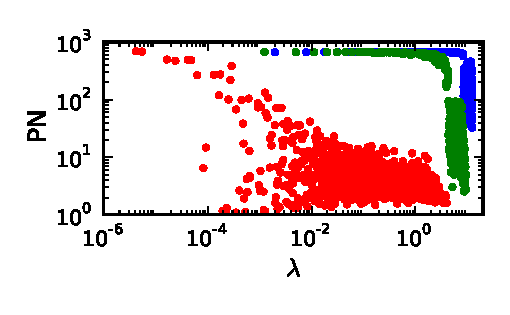
\includegraphics[width=0.99\linewidth]{pta_nopin}
    \caption{}\label{fig:PN_kottos_nopin}
  \end{subfigure}
  %
  \begin{subfigure}{.45\linewidth}\centering
    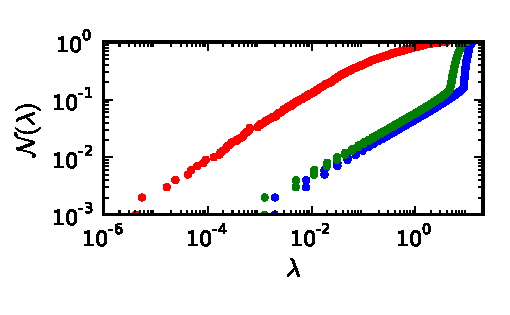
\includegraphics[width=0.99\linewidth]{pta_ev_nopin}
    \caption{}\label{fig:ev_dist}
  \end{subfigure}
  %\\ % end of row
  %
  \begin{subfigure}{.45\linewidth}\centering
    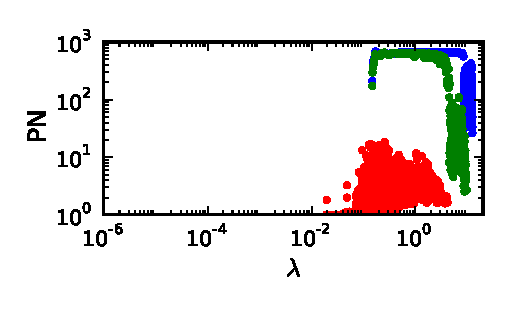
\includegraphics[width=0.99\linewidth]{pta_pin}
    \caption{}\label{fig:PN_kottos_pinning}
  \end{subfigure}     
  %
  \begin{subfigure}{.45\linewidth}\centering
     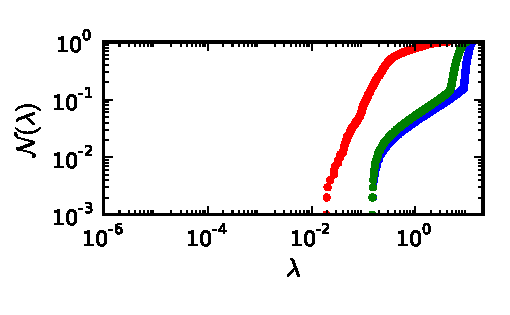
\includegraphics[width=0.99\linewidth]{pta_ev_pin}
  \caption{}\label{fig:ev_dist_pin}
   \end{subfigure}
  %
  \begin{subfigure}{.45\linewidth}\centering
    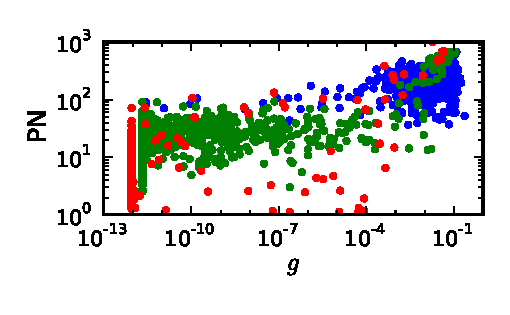
\includegraphics[width=0.99\linewidth]{pta_scatter_g}
    \caption{}\label{fig:PN_g_scatter}
  \end{subfigure}
  %
  \hspace*{\fill}
  \begin{subfigure}{.45\linewidth}\centering
    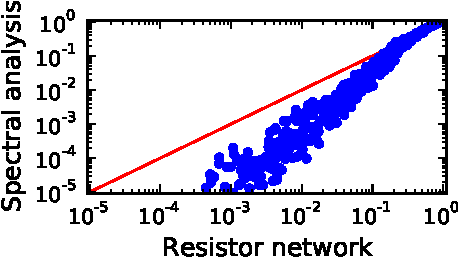
\includegraphics[width=0.99\linewidth]{ptsD_banded_scatter}
    \caption{}\label{fig:spectral}
  \end{subfigure}
  \\  % line end
  %
  \caption{For all the plots $N=1000$ and $b=5$. 
           In blue $\sigma=0.1$, green $\sigma=0.6$ and red $\sigma=10$, where higher
           $\sigma$ means more sparsity.
           %%%%
           In (\subref{fig:PN_kottos_nopin}) with low $\sigma$ (blue) we see two groups of PN values.
           This distinction is lost for higher $\sigma$ (red).
           %%
           In (\subref{fig:ev_dist}) we plot the cumulative distribution of
           the eigenvalues, presenting clear diffusive behavior, for any $\sigma$.
           %%%%%% pinning
           In (\subref{fig:PN_kottos_pinning}) and (\subref{fig:ev_dist})
           we see the effects of diagonal disorder (pinning)
           on the spectrum. We see clearly that the lowest eigenvalues 
           are affected, and their corresponding PN is much lower. The spectrum
           reveals sub-diffusive behavior.
           %%%g 
           In (\subref{fig:PN_g_scatter}) we compare the Thouless conductance
           $g$ with the participation number. 
           The presented points do seem to be correlated, but due to numerical issues,
           many values of $g$ are below the precision limit (seen as a vertical line in the plot), 
           up to $936$ from $1000$ for $\sigma=10$. 
           %%%%%  RESNET
           In (\subref{fig:spectral}) we compare $G_{DC\textrm{-spectral}}$ and $G_{DC\textrm{-Kirchoff}}$
           for a model with $b=10$ and $\sigma\in [0,80]$. They are correlated but unequal.
  }\label{fig:pta}
\end{figure}

\notbool{showfigure}{\end{comment}}{}




%%%%%%%%%%%%%%%%%%%%%%%%%%%%%%%%%%%%%%%%%%%%%%%%%%%%%%%%%
%%%%%%%%%   DTS
%%%%%%%%%%%%%%%%%%%%%%%%%%%%%%%%%%%%%%%%%%%%%%%%%%%%%%%%%

%%%%%%%%%%%%%%%%%%%%%%%%%%%%%
\section{Quantum spreading in a sparse banded Hamiltonian}\label{sec:dts}

In this section the numerical work was done in collaboration with
Eli Halperin and Tsampikos Kottos of Wesleyan university.


We define a Hamiltonian
\begin{align}
\mathcal{H}\ \ &=\ \ \epsilon B_{nm}\\
B_{nm} \ \ &= \ \ \textrm{random}[\pm]\eexp{-x}\qquad 0<|n-m| \le b \\
x \ \ &= \ \ \textrm{random} \ \in [0,\sigma]
\end{align}
that depends on three parameters, $\epsilon$, $b$ and $\sigma$. The $\sigma$
parameter controls the sparsity, and $b$ is the bandwidth, and $\epsilon$
defines the units of frequency.
In past works \cite{cohen_wave_2000,stotland_random-matrix_2010} it was deduced that the diffusion coefficient 
in a disordered banded system can be calculated as:
\begin{align}
D_0 \ \ &=\ \ \left[b\ \textrm{Var}[B_{nm}]\right]^{1/2}\ b^2\epsilon \\
\textrm{VAR}(B_{nm}) \ \ &=\ \ \int_0^\sigma \left(\pm \eexp{-x}\right)^2 \frac{dx}{\sigma}\ \ 
 =\ \  \frac{1-\eexp{-2\sigma}}{2\sigma} 
\end{align}

To question the validity of this result in the case of high sparsity,
we plot in \autoref{fig:D_of_s} the numerical results for $D$ divided by 
the speculated $D_0$. The results reveal that the sparsity affects the diffusion coefficient.
We see that as the system becomes more sparse, the diffusion coefficient is suppressed,
and as might be expected, the lower bandwidth ensembles are more
susceptible, as the system is more vulnerable to disconnections.


The next speculation is to use the suppression factor for sparse networks 
obtained in our previous work \autoref{sec:papers}:
%
\begin{align}
g_s(\sigma, b)\ \ &=\ \ \frac{D_{ERH}}{D_{\textrm{linear}}}\ \ =\ \ 
\frac{  \left(1+\frac{n_c}{b}\sigma\right)\eexp{-\frac{n_c}{b}\sigma}
                                              - \eexp{-4\sigma}}{1-\eexp{-4\sigma}}\\
\textrm{With } n_c\ &\approx 2
\end{align}

In \autoref{fig:d_vs_g} we plot in log-log scale $\frac{D}{D_0}$ vs $g_s$, assuming a relation:
%
\begin{align}
\frac{D}{D_0}\ \ \approx \ \ C\ \ g_s(\sigma,b)^\gamma
\end{align}
It seems that this scaling hypothesis fails, as the 3 lines do not coincide.


\begin{figure}
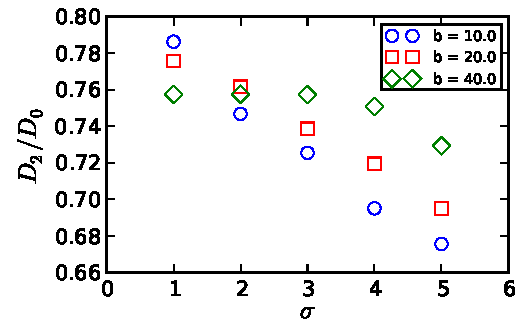
\includegraphics{dts_D2}
\caption{The transient diffusion coefficient for quantum spreading in
a banded sparse network. The ratio $D/D_0$ between the numerical diffusion 
coefficient and the expected value decreases as $\sigma$ increases. The effect
is stronger for low bandwidth.}\label{fig:D_of_s}
\end{figure}


\begin{figure}
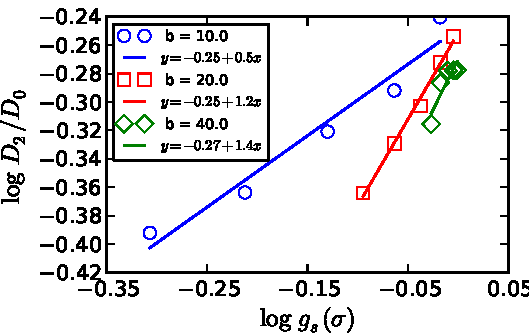
\includegraphics{dts_D2_vs_gs_loglog}
\caption{Scaled $D$ vs $g_s$. }\label{fig:d_vs_g}
\end{figure}
